%%%%%%%%%%%%%%%%%%%%%%%%%%%%%%%%%%%%%%%%%%%%%%%%%%%%%%%%%%%%%%%%%%%%%%
% Problem statement
\begin{statement}[
  problempoints=100,
  timelimit=3 sekunde,
  memorylimit=512 MiB,
]{Šeširi}

Srednjoeuropska informatička olimpijada (CEOI) ove se godine održava u Lijepoj
Našoj. Natjecatelji su dodatno uzbuđeni zbog najpoznatije hrvatske tradicije na
informatičkim olimpijadama. Naravno, radi se o darivanju šeširića s
prepoznatljivim ``kockastim'' uzorkom.

Ipak, gospodin Malnar odlučio je stati na kraj još jednoj tradiciji. Ove će se
godine dijeliti jednobojni šeširići, obojeni u crvenu ili bijelu boju. Gospodin
Malnar nije donio ovu odluku tek tako, već je to dio pomno promišljenog plana.

Naime, Malnar zna da će se u nekom trenutku na istom mjestu naći $N$ mladih
informatičara te da će svaki od njih na glavi nositi crveni ili bijeli
šeširić.  Naravno, svaki će informatičar vidjeti sve šeširiće osim svojeg te
će, po običaju, svi istovremeno viknuti koje boje misle da je njhov šeširić.

Svi informatičari koji pogode boju svojeg šeširića za nagradu će otići na večeru
s gospodinom Malnarom. No, gospodinu
Malnaru jako je stalo do toga da na večeri obje boje šeširića budu dovoljno
zastupljene. Rekao im je da od svih $b$ informatičara s bijelim
šeširićem \textbf{barem $\lfloor b/2 \rfloor$} njih mora pogoditi svoju boju, te od svih
$c$ informatičara s crvenim šeširićem \textbf{barem $\lfloor c/2 \rfloor$} njih mora
pogoditi svoju boju, jer inače neće nikoga voditi na večeru.

Pomozite mladim informatičarima pronaći strategiju koja će osigurati da uvjet
gospodina Malnara bude ispunjen za svaki mogući raspored šešira.

%%%%%%%%%%%%%%%%%%%%%%%%%%%%%%%%%%%%%%%%%%%%%%%%%%%%%%%%%%%%%%%%%%%%%%
% Input
\subsection*{Ulazni podaci}
U prvom i jedinom retku je prirodan broj $N$, broj informatičara.

%%%%%%%%%%%%%%%%%%%%%%%%%%%%%%%%%%%%%%%%%%%%%%%%%%%%%%%%%%%%%%%%%%%%%%
% Output
\subsection*{Izlazni podaci}

Informatičari su označeni prirodnim brojevima od $1$ do $N$.
Neka je $s_i$ znak koji predstavlja boju šeširića $i$-tog informatičara, \texttt{B}
za bijelu odnosno \texttt{C} za crvenu boju.

U $i$-tom retku treba ispisati niz od $2^{N-1}$ znakova \texttt{B} i \texttt{C}
koji opisuju strategiju $i$-tog informatičara.
Označimo taj niz znakova s $x_i$.
Informatičar će pogledati šešire ostalih, i situaciju koju vidi opisati nizom
znakova $y_i = s_1 \dots s_{i-1} s_{i+1} s_N$. Zatim će odrediti redni broj $k_i$ tog niza
znakova među abecedno poredanim svim nizovima znakova \texttt{B} i \texttt{C} duljine $N - 1$.
Ako je $k_i$-to slovo u njegovoj strategiji $x_i$ jednako \texttt{B}, reći će
``bijela!'', odnosno ako je \texttt{C} onda će reći ``crvena!''.

Za dodatno pojašnjenje pogledajte probne primjere.

%%%%%%%%%%%%%%%%%%%%%%%%%%%%%%%%%%%%%%%%%%%%%%%%%%%%%%%%%%%%%%%%%%%%%%
% Scoring
\subsection*{Bodovanje}
{\renewcommand{\arraystretch}{1.4}
  \setlength{\tabcolsep}{6pt}
  \begin{tabular}{cc'cc'cc}
      Testni primjer & Broj bodova & Testni primjer & Broj bodova & Testni primjer & Broj bodova \\ \midrule
      $N = 4$ & 7 & $N = 9$ & 7 & $N = 14$ & 6 \\
      $N = 5$ & 7 & $N = 10$ & 7 & $N = 15$ & 6 \\
      $N = 6$ & 7 & $N = 11$ & 7 & $N = 16$ & 6 \\
      $N = 7$ & 7 & $N = 12$ & 7 & $N = 17$ & 6 \\
      $N = 8$ & 7 & $N = 13$ & 7 & $N = 18$ & 6 \\
\end{tabular}}


%%%%%%%%%%%%%%%%%%%%%%%%%%%%%%%%%%%%%%%%%%%%%%%%%%%%%%%%%%%%%%%%%%%%%%
% Examples
\subsection*{Probni primjeri}
\begin{tabularx}{\textwidth}{X'X}
\sampleinputs{test/sesiri.dummy.in.1}{test/sesiri.dummy.out.1} &
\sampleinputs{test/sesiri.dummy.in.2}{test/sesiri.dummy.out.2}
\end{tabularx}

\textbf{Pojašnjenje probnih primjera:} 
\begin{figure}[H]
    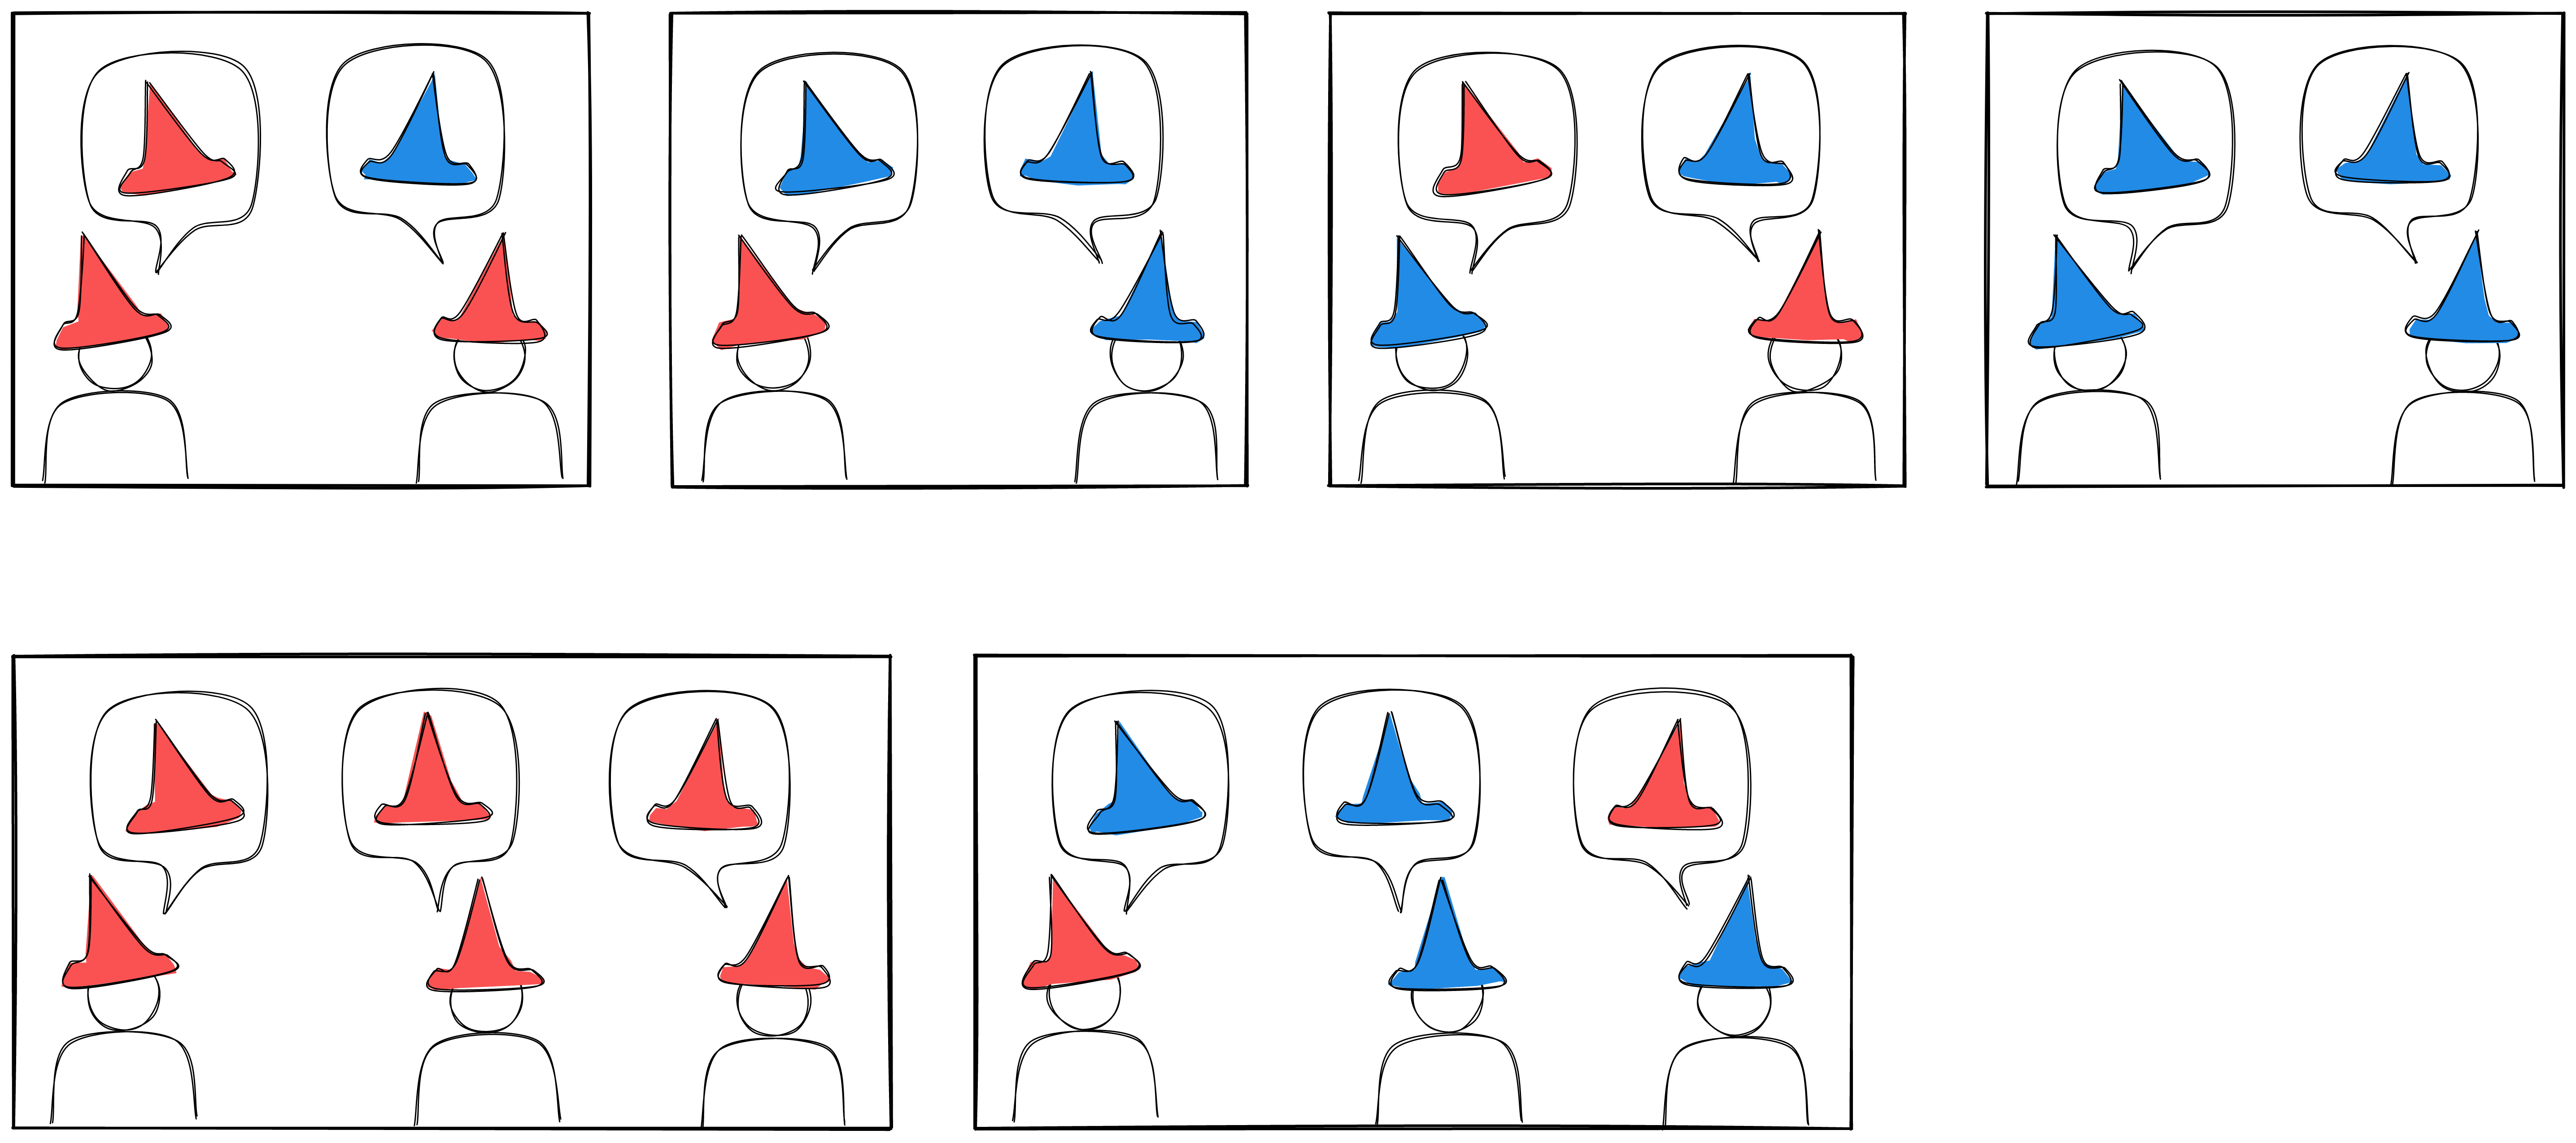
\includegraphics[width=0.95\textwidth]{img/sesiri_dummy.excalidraw.png}
\end{figure}

Prvi redak slike prikazuje sva četiri moguća slučaja u prvom primjeru.

Drugi redak slike prikazuje dva moguća slučaja u drugom primjeru.

Prvi slučaj:
$$
\begin{array}{lccccccccc}
    1 & & s_1 = \texttt{C} &          & x_1 = \texttt{CC} &          & k_1 = 4 &          & \texttt{C} \\
    2 & & s_2 = \texttt{C} & \implies & x_2 = \texttt{CC} & \implies & k_2 = 4 & \implies & \texttt{C} \\
    3 & & s_3 = \texttt{C} &          & x_3 = \texttt{CC} &          & k_3 = 4 &          & \texttt{C} \\
\end{array}
$$
Drugi slučaj:
$$
\begin{array}{lccccccccc}
    1 & & s_1 = \texttt{C} &          & x_1 = \texttt{BB} &          & k_1 = 1 &          & \texttt{B} \\
    2 & & s_2 = \texttt{B} & \implies & x_2 = \texttt{CB} & \implies & k_2 = 3 & \implies & \texttt{B} \\
    3 & & s_3 = \texttt{B} &          & x_3 = \texttt{CB} &          & k_3 = 3 &          & \texttt{C} \\
\end{array}
$$

% We're done

\end{statement}

%%% Local Variables:
%%% mode: latex
%%% mode: flyspell
%%% ispell-local-dictionary: "croatian"
%%% TeX-master: "../hio.tex"
%%% End:
